As was described in section \ref{subsection:dl} the choice of the model architecture fell onto the UNet structure. Here a detailed description of the architecture and the different layers used will be provided. An architecture used in this research was chosen based on paper \cite{Lachance_2020}. The input to this network is a $256 \times 256$ pixel DIC image that should already be preprocessed based on the corresponding preprocessing pipeline to the desired organelle. Specifications about different preprocessings are described separately in the next subsections dedicated to different organelles.

The encoder part of the UNet (Figure \ref{fig:unet}) compresses the spatial dimensions of the image step by step (the spatial dimension size is denoted by a number on the left of each green block) into tensors or so-called feature maps with an increasing amount of filters (the number of filters is denoted on top of each green block). This allows to reduce the spatial information in the image and capture semantics. The decoder part on the contrary decompresses feature maps gradually increasing the amount of spatial information in tensors and reducing the number of filters. All convolutional layers use convolutions of size $3 \times 3$ with the corresponding number of filters. Downsampling in encoder reduces the spatial dimension twice during each step and is implemented using max-pooling with a size of $2 \times 2$. Upsampling in decoder increases the spatial dimension also twice during each step and is implemented using transposed convolutions with a size of $2 \times 2$. After the first convolution that follows each max-pooling step a batch normalization layer was used as it is well-known for speeding up the training process (\cite{Ioffe_2015}). It should not be forgotten however that the use of batch normalization might sometimes be dangerous due to the hidden information leaks that are being induced (\cite{fetterman}). Additionally, dropouts were used for example for actin predictions as the model would encounter overfit quite easily there, however in the default architecture dropouts are not present. That is another thing that differentiates this architecture from the original one in \cite{Lachance_2020} paper. The last layer of the UNet here is a sigmoid activation function.
\begin{figure}[htb]
	\begin{center}
		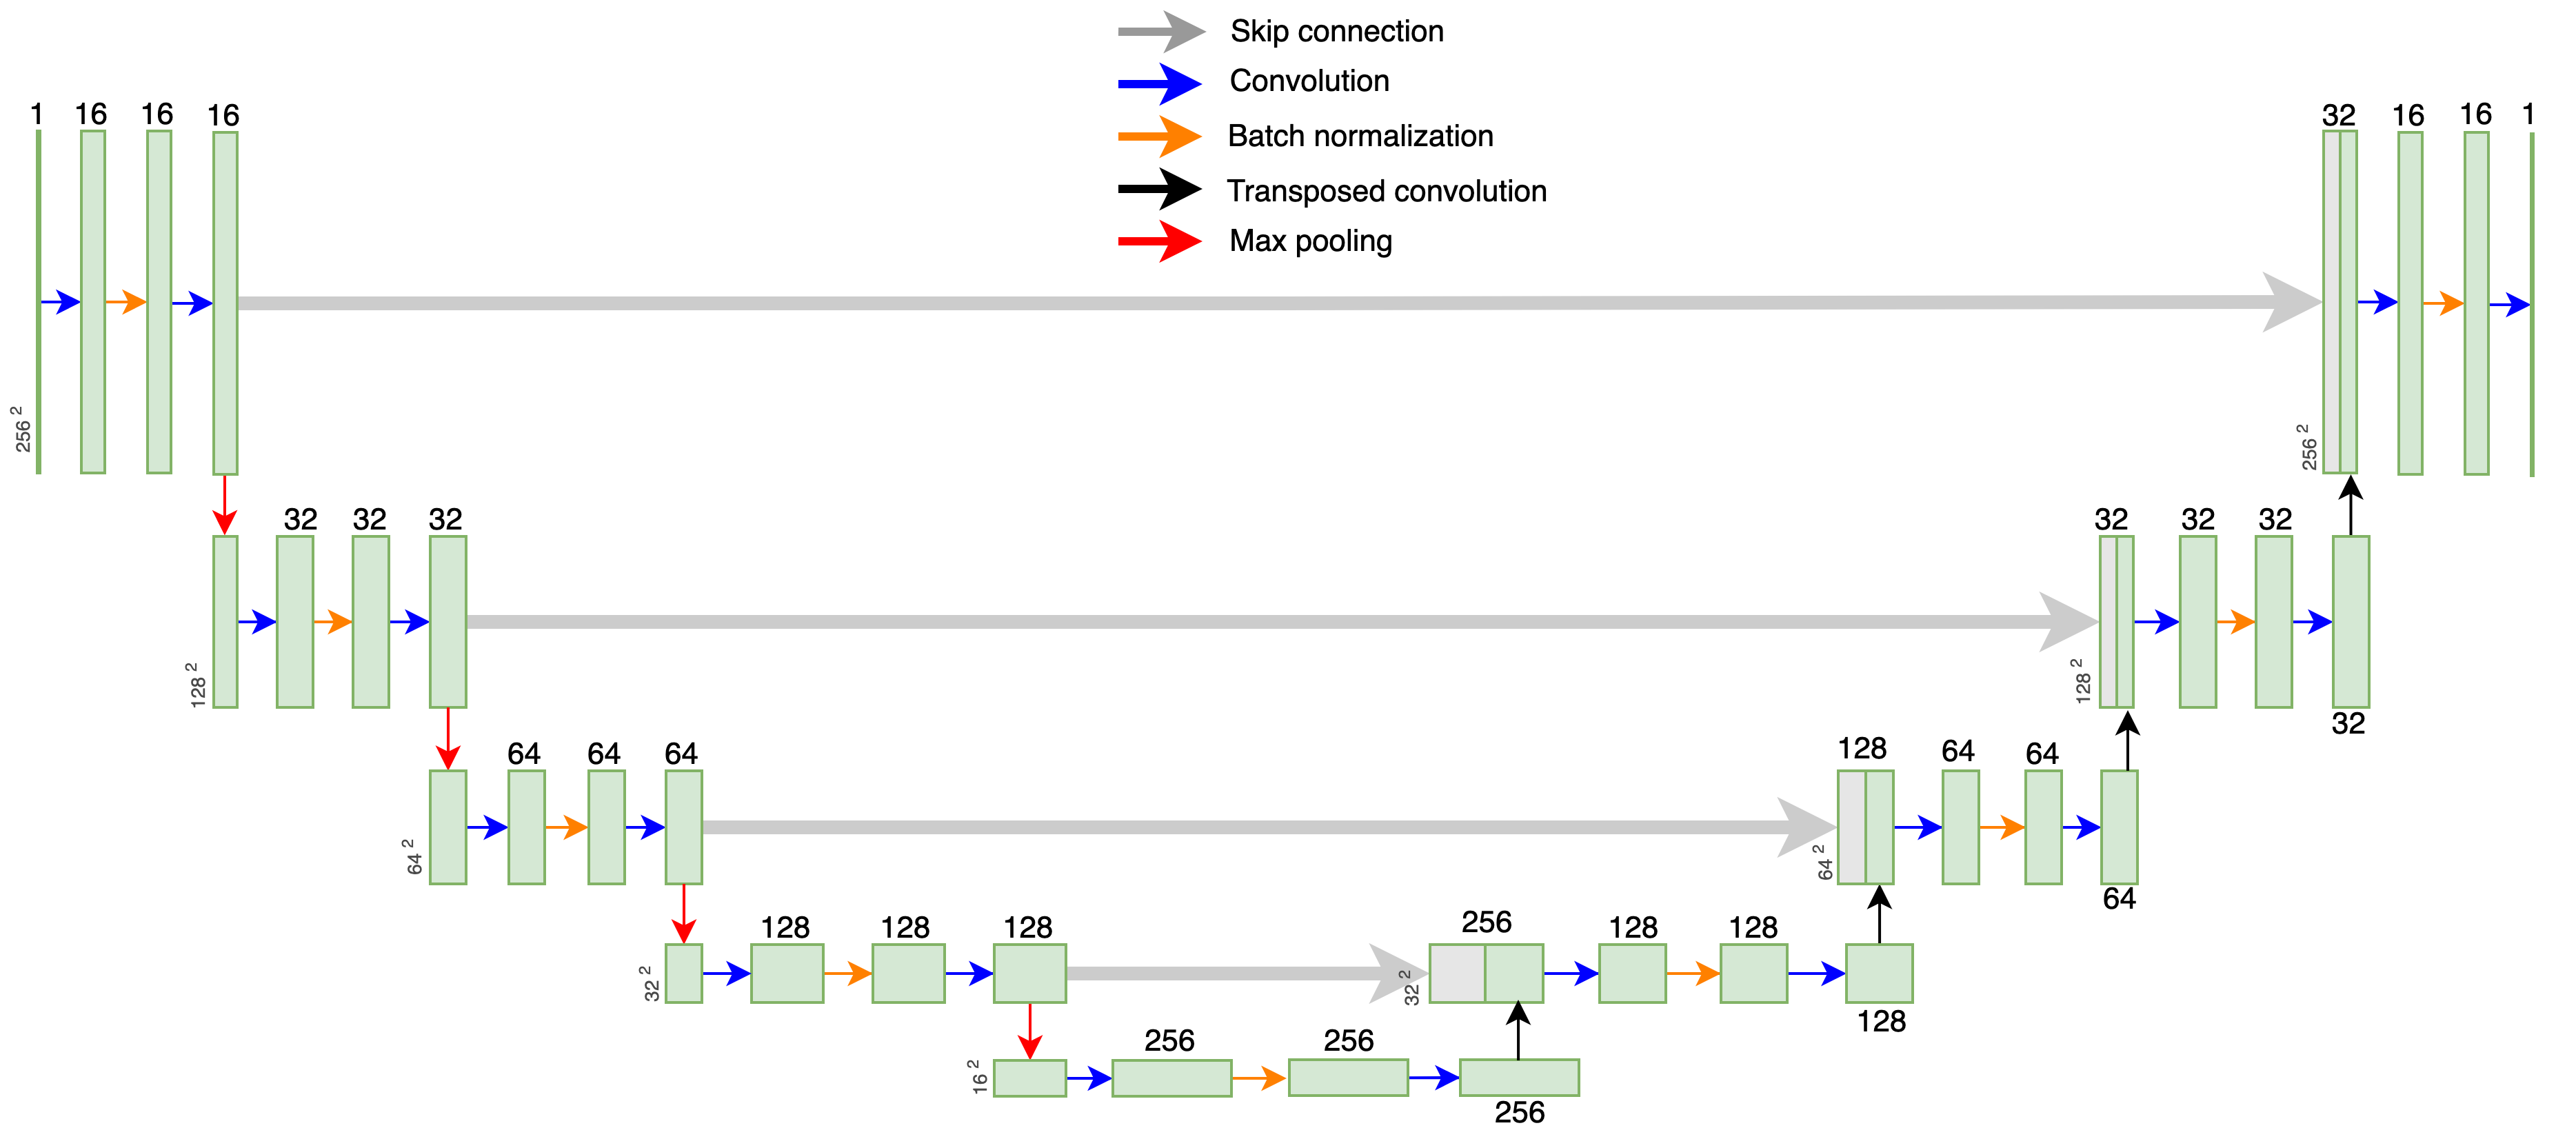
\includegraphics[width=\linewidth]{bilder/Unet.png}
		\caption{UNet}\label{fig:unet}
	\end{center}
\end{figure}

There is a space for potential improvements regarding the model architecture used in this research: for example, \cite{Cheng_2021} recommend to use special dense-blocks after each convolutional layer. They consist of another 3 convolutional layers with 24 filters, batch normalization layer and ReLU activations each. This could potentially facilitate efficient training of the model, still most probably the efficience comes mostly from batch normalization layers that are already used in our architecture. Nevertheless the idea of using a bigger model such as one in \cite{Cheng_2021}, or more specifically a model with more filters, indeed improves the predictions (shown in Section [TODO ref section]). That that leaves room for further research and improvements regarding the size of the model and the additional use of dense-blocks.

An interesting question that arises here automatically is: what do UNet embeddings (output tensors from the encoder) represent? There is a big difference between any representation learning network such as an autoencoder and a UNet --- a UNet model uses skip-connections that allow to propagate information between its encoder and a decoder. This means that embeddings do not contain purely semantic information, because essentially the network is not pushed towards compressing the information severely (as an autoencoder would do), but it should only extract information relevant for segmentation features. One of the questions solved in this work was whether or not UNet embeddings are clustering based on the following classes: cell phenotypes, any kind of corruption within the data. For example, it would be very useful to be able to not only predict the data itself, but also to say whether the prediction is reliable or not. The initial hypothesis here stats that if the predictions are not of a good enough quality this would also be reflected in the embeddings.